

\section{Architecture}


\speculake malware is comprised of two independent programs: a payload program, and a
trigger program. Both are installed on the victim's computer (e.g. via trojan, remote
exploit, or phishing), and must run simultaenously on the same physical CPU. We
note that the constraint of running programs on the same CPU is not a signifcant
burden: \texttt{taskset} can be used to limit a process to a core, or if not
available, the attacker can simply run multiple copies of the trigger or payload
program to coerce the OS scheduler to assign a payload/trigger pair to the same
core.

At a high level, the trigger program performs a series of indirect jumps in a
loop, training the branch predictor to this pattern. Meanwhile, the
payload program performs a subset of this jump pattern, then forces the CPU to
speculate by stalling the resolution of an indirect branch via a slow memory
read. The CPU will (mistakenly) predict the jump to follow the pattern performed
by the trigger program, and speculatively execute that destination in the
payload program.

\subsection{Indirect jumps}

Indirect branch predictors allow the CPU to predict the destination address of a
branch based solely off its source address and a brief history of previous
branch sources and destinations. While the inner-working details of modern CPU
branch predictors are proprietary, it is possible to reverse engineer parts of
their behavior, which we do in \speculake.

We created a simple trigger program that performs a series of 32 indirect jumps,
using the \texttt{jmpq *\%rax} instruction. Between each jump, we increment
\texttt{\%rax} to account for the number of bytes between jumps. For the last
jump, we load a function pointer into \texttt{\%rax} and do a final indirect
jump using \texttt{callq \%rax}.


In our payload program, we first perform the same 32 indirect jumps. We ensure
the source address of these jumps is the same as in the trigger program by
manually defining their containing function at a fixed address inside a linker
script. We also do the final indirect call to a function pointer, but with two
differences. First, the destination of the function pointer is a different
address, and second, the location of the function pointer in memory is uncached.
This forces the CPU to predict the destination of the indirect call, which it
predicts to be the destination of the function pointer in trigger program. In
the payload program, we purposefully place code at this address which acts as
the \emph{speculative entry point}. Even though the in-order execution of
payload program never executes or even reads from this address, the CPU will
briefly execute instructions there speculatively.

Eventually, the dereference of the uncached function pointer in payload program
will be resolved, and the CPU will recognize it has incorrectly predicted the
destination of its \texttt{callq} instruction. The results from the speculative
entry point instructions will be discarded, and the CPU will continue executing
from the correct destination. However, as the speculative code changes what is
loaded into the cache based on its results, it can covertly communicate its
results to the ``real world'' program.


TODO: Note that returns can also be indirect jumps, and rets/jmpq can be mixed
to a certain extent...need to document/quantify how much mixing can be done
still.


\begin{figure}[t]
    \centering
        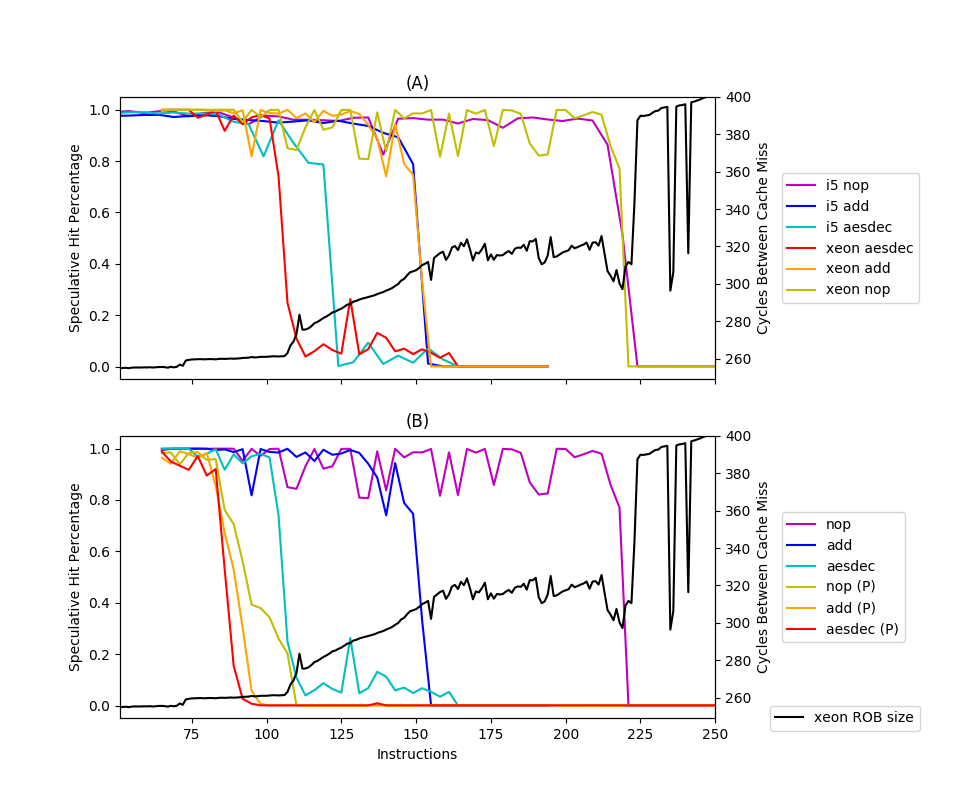
\includegraphics[width=0.5\textwidth]{figures/speculative_measurements.png}
    \caption{The speculative primitive allows for a limited number of instructions
        to be completed speculatively, dependent on multiple factors. A) The 
        processor generation determines the maximum ROB size and PRF capacity,
        however intel xeon E3-1270(warm colors) and i5-7200U both (cool colors) 
        perform similarly for comparable instructions. B) Because trigger and 
        payload processes must share cpu resources they must be performed on 
        the same hyperthread or associated parity hyperthreads. Processes on
        the parity hyperthreads (warm colors) denoted by (P) accomplish a 
        significantly lower number of instructions as compared with processes 
        on the same hyperthread (cool colors).}
    \label{fig:spec-capacity}
\end{figure}

\subsection{Limits of Speculative Execution}
We performed several experiments to investigate how much computation can be done
speculatively. We performed these experiments on an Intel Xeon-1270, as well as 
an intel i5-7200U to verify the results across processor generations. 

Speculative branching is not a new feature in processors~\cite{branching-hist}, 
and it has been integrated in multiple generations of commodity processors today. 
Accordingly speculative instruction capacity has fairly well defined limits, in 
line with known features of processor designs. We have determined that features 
like reorder buffers (ROB), physical register file (PRF), and cache miss timing
determines a strong limit on the number of instructions that can be accomplished
speculatively. 

\subsubsection{Reorder Buffer Capacity} \label{sssec:ROB}
To determine these limits we first measured the capacity of the reorder buffer
using the method outlined by~\cite{intel-rob-capacity}. By performing two cache loads
with a variable number or instructions between them and watching the amount of 
time taked to complete this loop we can find a definitive number of instructions
at which the second cache access is outside of the ROB. Figure~\ref{fig:spec-capacity}
shows this step function at ~220 instructions for both Sandy Lake and Kaby Lake 
generation processors. 

\subsubsection{Cache Miss Duration}
When executing instructions speculatively we rely on a load from a cache line that
has recently been evicted. We have examined the number of cycles a
cache miss takes to return by artificially evicting an item from cache and timing 
a request for that specific item. The distribution of cycle counts can be seen in
Figure~\ref{fig:cache-miss}, along with the CDF. For a large majority of cases, 
an item evicted from cache will have 300 clock cycles and often much more. 

\subsubsection{Speculative Instruction Capacity}
To verify that the ROB defines an upper limit for speculative instruction capacity
we instrumented the trigger and payload to test variable length target functions. 
In addition we tested whether instruction complexity or data dependencies impact
the maximum work that can be completed. We found that the processor can identify 
some operations that have no effect on output registers and allows them to use the 
entire size provided by the ROB, as determined in section~\ref{sssec:ROB}. This includes 
idomatic no-ops and zero idioms, which have no reliance on register values, 
for example the instruction \textit{xchg \%rax \%rax} and \textit{xor \%rax, \%rax}. 
However, if an instruction is a potential data hazard, it must use an entry in the PRF
until it reaches the correct stage in the execution pipeline. In this case, the number 
of instructions is limited by the PRF entries available.

Most notably instructions making use of the extended x86 registers are still
valid within speculative context. Specifically Intel's hardware accelerated AES-NI
encryption and decryption instructions, which make use of the 128 bit registers.
As shown in Figure~\ref{fig:spec-capacity}, speculative environments can complete
a significant number of AES rounds -- more than enough to decrypt a full block 
using AES-CBC. We investigate the use of AES instructions in the spculative environment
further in Sections~\ref{subsec:decryption}.

\medskip

When executing speculatively, the number of instrutions completed 
will almost never be limited by cache miss duration. Instead
ROB size and processor mechanisms for resolving 
data dependencies define an upper boundary. 

% TODO: 
% - Highlist instruction signal variablity (add v mul v aesdec v nop)?
% - Limitation is in the ROB (cite other work that supports this)
% - MORE PROCESSORS for testing?
% - ARM?


\begin{figure}[h]
    \centering
        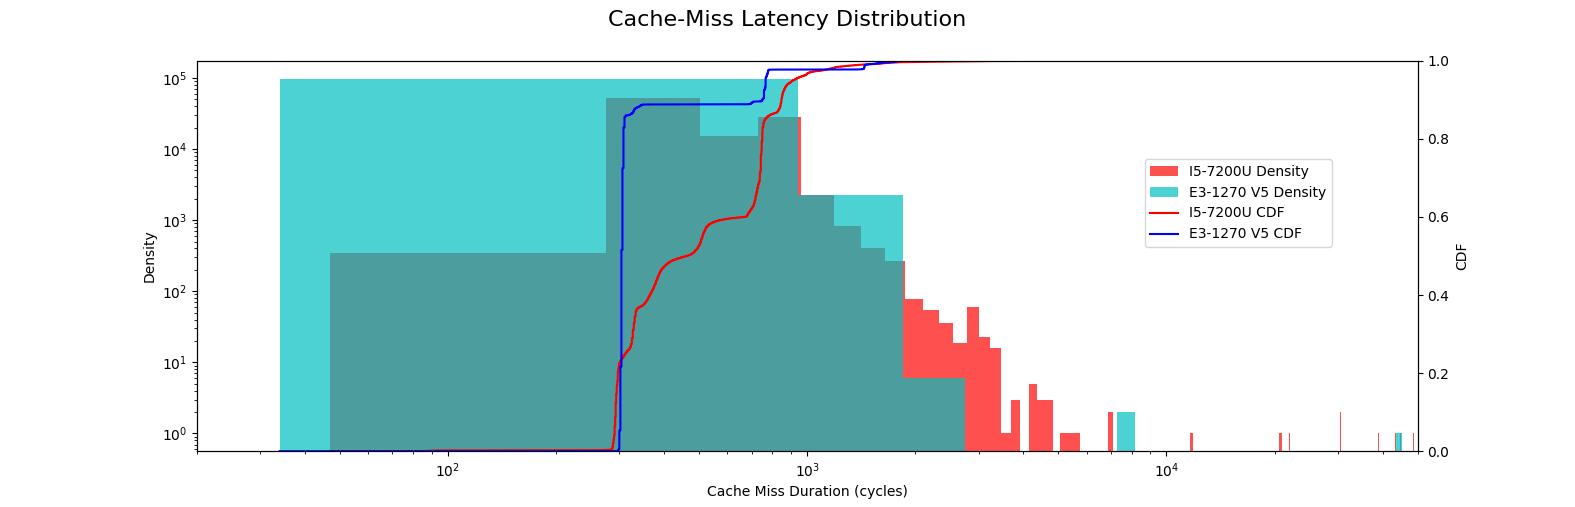
\includegraphics[width=0.5\textwidth]{figures/cache_miss_dist}
    \caption{}
    \label{fig:cache-miss}
\end{figure}

\subsection{Speculative Primitive}

We summarize our findings into a \emph{speculative primitive}, which allows us to
speculatively (and covertly) perform approximately TK:150 arbitrary
instructions, and communicate a short (e.g. single byte) result to the real
world via a cache side channel. These speculative instructions are able to read
from any real-world memory or registers, but they cannot perform updates or
writes directly. To update memory, the speculative instructions must communicate
to the real world through a cache side channel.

We note a performance tradeoff between the size of communication (e.g. 4 bits vs 8
bits) and the time it takes the real world to recover the result from the side
channel. Using Prime+Probe~\cite{prime-probe} as our cache side channel,
recovering the result requires accessing all elements in an array exponential in
the size of the result (e.g. $2^8$ array reads to recover an 8-bit result). 
Therefore, there is a
performance advantage for keeping the size of the result small, and communicating
out small pieces of information that are aggregated by the real world.


%%%%%%%%%%%%%%
